\section{Écarts à la planification}
\label{sec:ecarts}

Durant l'implémentation de Glasir, plusieurs évenements sont venus impacter la planification initialement prévue du projet. Pour rendre compte de cela, les diagrammes de Gantt d'avant et après implémentation sont présentés aux figures 
\BK{{\sc figures}}~\ref{fig:planifInit} et ~\ref{fig:planif}. 
\BK{Il ne faut pas mettre d'espece avant le symbole de 'tilde'}
Vont être détaillés ci-après les changements et faits majeurs du point de vue de la planification du projet. 

\subsection{Gestion du temps}

L'un des premiers constats que l'on peut énoncer maintenant l'implémentation terminée, est que nous avions de manière générale légèrement surévaluée la durée des tâches, comme il est possible de la remarquer en comparant les figures ~\ref{fig:planifInit} et  ~\ref{fig:planif}
\BK{{\sc figures}~\ref{fig:planifInit} et~\ref{fig:planif}.}
. Cette surévaluation nous a permis de gagner du temps, qui a été utilisé pour pousser plus loin certaines fonctionnalités du logiciel ou bien pour en créer de nouvelles, mais également pour surmonter les difficultés que nous avons rencontrées.

Ce supplément de temps nous a permis de gérer la sauvegarde de plus d'une modification de l'arbre dans ADTool, et permet donc d'annuler plusieurs actions grâce à la fonctionnalité Undo, au lieu d'une seule comme annoncée initialement.

Toujours sur ADTool, ce temps supplémentaire a permis plusieurs améliorations mineures, comme le nommage des fenêtre, mais nous a surtout permis de développer une version \og Viewer \fg d'ADTool, dont l'intérêt est décrit en section ~\ref{sec:decisions} \BK{{\sc section}~\ref{sec:decisions}}.

Enfin, cela nous aura servi à gérer les difficultés non attendues que nous avons pu avoir dans les algorithmes des modules de Glasir, sans faire prendre de retard au projet. Nous avons même été en mesure de fournir une version plus intelligente du filtre qu'annoncée, qui est capable de trouver les noeuds incorrects même en dessous de noeuds conjonctifs.  
\BK{n\oe{}uds (voir sources LaTex pour la commande utilisée)}

\subsection{Décisions d'implémentation}
\label{sec:decisions}

\BK{On ne commence pas une phrase avec 'mais'. De plus vous parlez d'une 'avancée'. Quelle avancé?}
Mais malgré cette avance, nous avons également été confronté \BK{confrontés?} à des difficultés que ce temps supplémentaire ne nous a pas permis de gérer. Nous avons en effet du abandonner deux éléments du logiciel tel qu'initialement prévu : la fonctionnalité d'affichage multi-paramètres sous ADTool et l'intégration complète d'ADTool au sein de Glasir.

L'affichage multi-paramètres, que nous estimions être une fonctionnalité relativement simple à implémenter, s'est en réalité révélé infaisable dans le cadre de ce projet. En effet, ADTool ayant été conçu autour d'une classe de fenêtre d'affichage a un seul paramètre, et dont tout le code dépend, les modifications nécessaires à l'implémentation de cette fonctionnalité nous auraient demandé de revoir presque l'intégralité du code d'ADTool, ce qui compte tenu de la taille du soft 
\BK{la taille de quoi? :)}
n'est pas \BK{n'a pas été} possible dans le cadre de ce projet. De la même manière que nous ne pouvions pas intégrer les fonctionnalités d'analyse à ADTool sans avoir à le réécrire intégralement.

L'intégration complète d'ADTool au sein de Glasir a quant à elle été abandonnée après de longs et infructeux essais. 
\BK{La phrase précédente est très négative}
Nous n'avons simplement pas pu trouver de méthodes permettant l'éxecution d'un thread Java au sein d'un processus C\#. Pour remédier à cette impasse, nous avons mis au point une version \og Viewer \fg de ADTool, où toutes les fonctionnalités de création et de modification d'arbres sont désactivées. Cette version nous permet de pouvoir utiliser ADTool en tant que processus extérieur à Glasir, sans craindre de perdre l'utilisateur avec des modifications d'arbres sous ADTool ignorées de Glasir.  

    \begin{figure}[H]
        \centering
        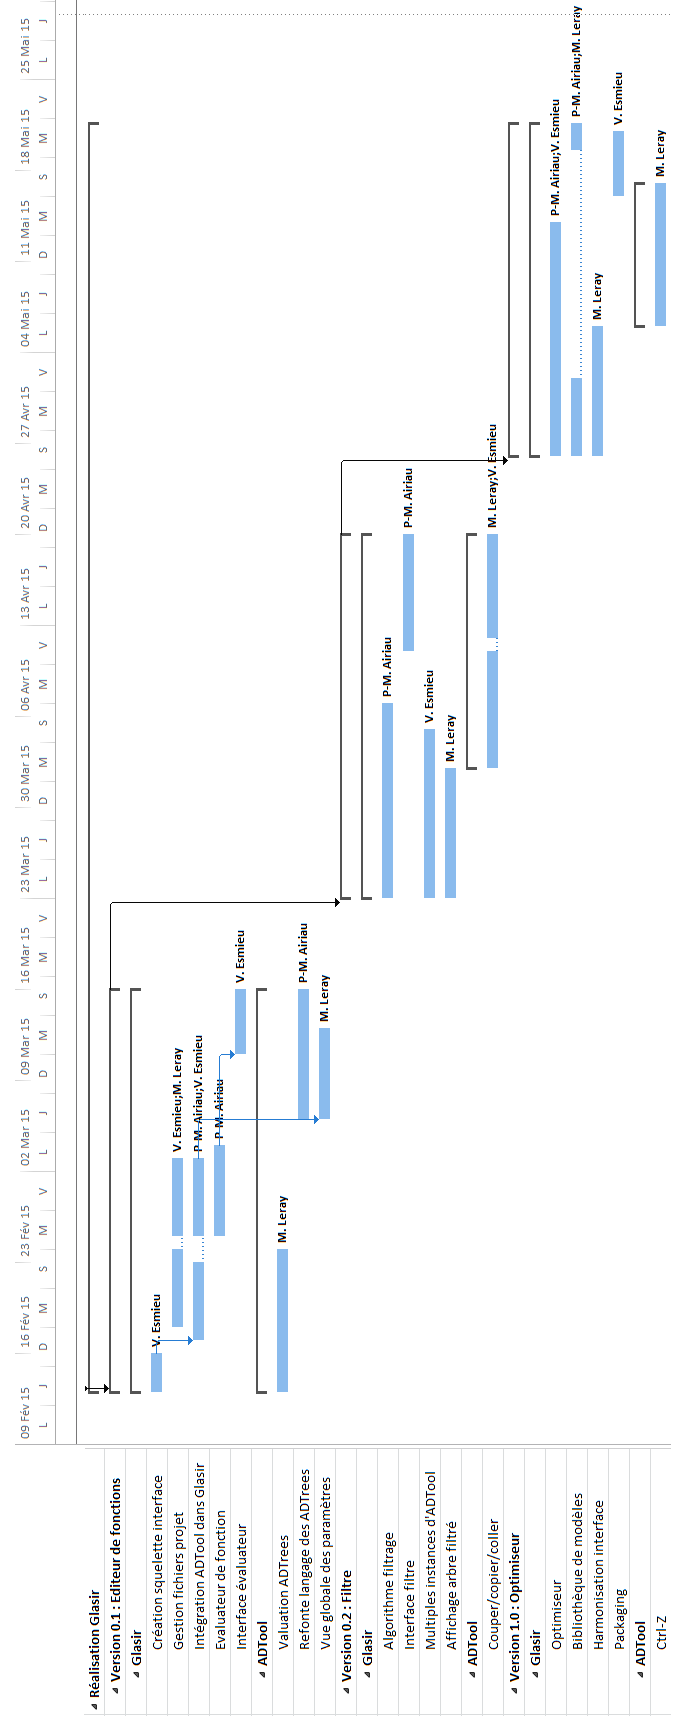
\includegraphics[height=1.6\textwidth]{figure/planifInit.png}
        \caption{Diagramme de Gantt au début du projet\glasir{}. \BK{espace entre projet et \glasir{}}}
        \label{fig:planifInit}
    \end{figure}

    \begin{figure}[H]
        \centering
        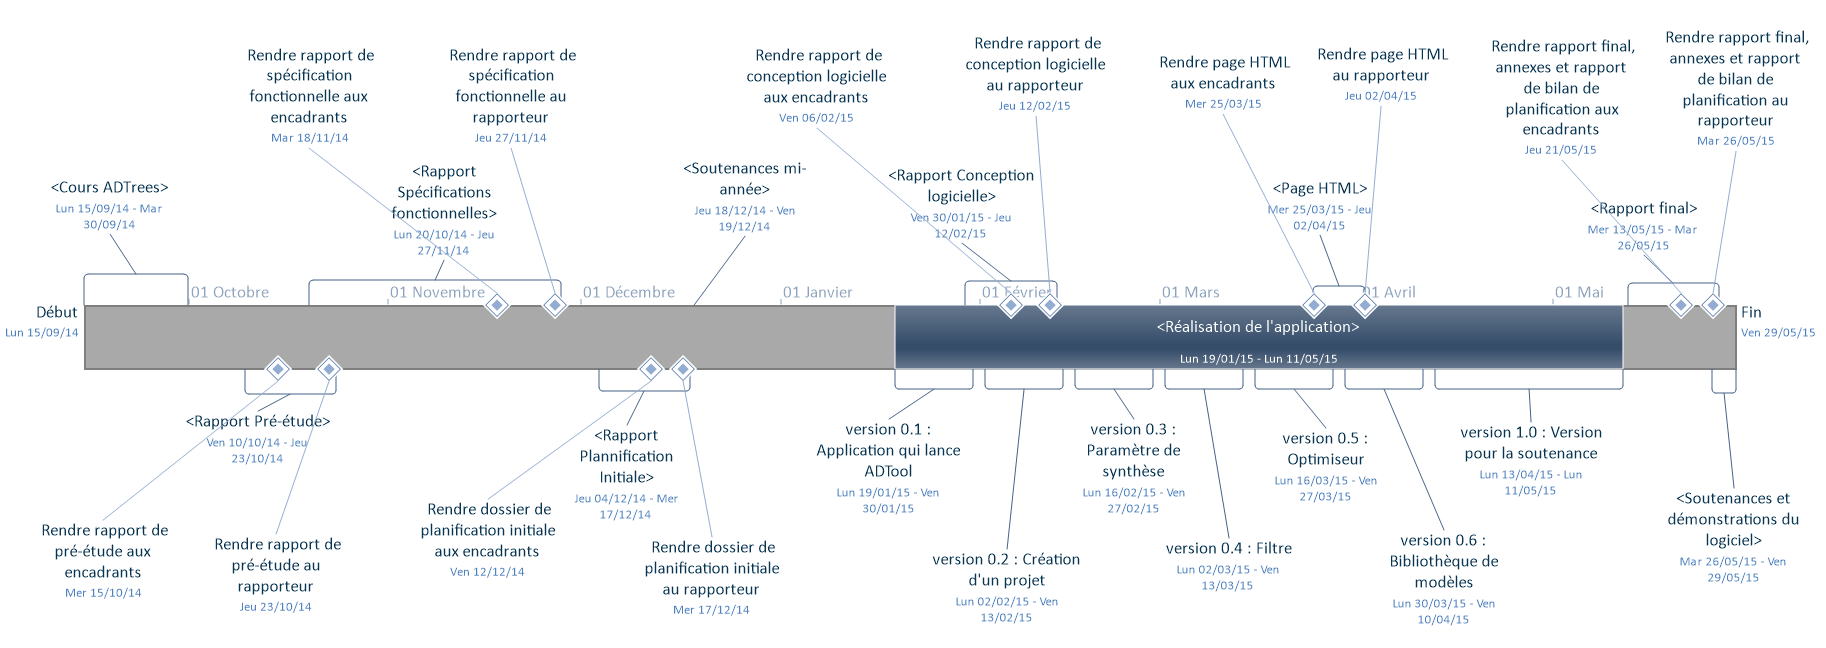
\includegraphics[height=1.6\textwidth]{figure/planification.png}
        \caption{Diagramme de Gantt à la fin du projet\glasir{}. \BK{espace entre projet et \glasir{}}}
        \label{fig:planif}
    \end{figure}





